\documentclass[oneside,senior,etd]{BYUPhysForDegree}

\usepackage[T1,T2A]{fontenc} % gleb

\usepackage[utf8]{inputenc}
\usepackage{rotating} 

%json
\usepackage{minted}

\usepackage[russian]{babel}
\usepackage{amsfonts} % Пакеты для математических символов и теорем
\usepackage{amstext}
\usepackage{amssymb}
\usepackage{amsthm}
\usepackage{graphicx} % Пакеты для вставки графики
\usepackage{subfig}
\usepackage{color}
\usepackage[unicode]{hyperref}
\usepackage[nottoc]{tocbibind} % Для того, чтобы список литературы отображался в оглавлении
\usepackage{algorithmic} % Для записи алгоритмов в псевдокоде
\usepackage{algorithm}
\usepackage{verbatim} % Для вставок заранее подготовленного текста в режиме as-is
\usepackage{listings}

% =================================================
% https://www.overleaf.com/learn/latex/Code_listing
% =================================================

\usepackage{xcolor} 

%New colors defined below
\definecolor{codegreen}{rgb}{0,0.6,0}
\definecolor{codegray}{rgb}{0.5,0.5,0.5}
\definecolor{codepurple}{rgb}{0.58,0,0.82}
\definecolor{backcolour}{rgb}{0.95,0.95,0.92}

%Code listing style named "mystyle"
\lstdefinestyle{mystyle}{
  backgroundcolor=\color{backcolour}, commentstyle=\color{codegreen},
  keywordstyle=\color{magenta},
  % numberstyle=\tiny\color{codegray},
  stringstyle=\color{codepurple},
  basicstyle=\ttfamily\footnotesize,
  breakatwhitespace=false,         
  breaklines=true,                 
  captionpos=b,                    
  keepspaces=true,                 
  % numbers=left,                    
  % numbersep=5pt,                  
  showspaces=false,                
  showstringspaces=false,
  showtabs=false,                  
  tabsize=2
}

%"mystyle" code listing set
\lstset{style=mystyle}

% =================================================
% =================================================







\usepackage{commath}
\newcommand\Tau{\mathcal{T}}
\newcommand{\R}{\mathbb{R}}
\usepackage{color}
\usepackage[colorinlistoftodos, prependcaption]{todonotes}
\usepackage{multirow}
\newcommand*{\MyIndent}{\hspace*{0.2cm}}%

\Chair{Кафедра суперкомпьютеров и квантовой информатики}
\Lab{~}
\Year{2023}
  \Month{Август}
  \City{Москва}
  \AuthorText{Автор}
  \Author{Скрябин Глеб Денисович}
  \AuthorEng{Gleb Skryabin}
  \AcadGroup{423}
  \TitleTop{Разработка технологий 3D визуализации}
  %\TitleMiddle{}
  \TitleBottom{информационных графов алгоритмов} % leave empty if you don't need it
  \TitleTopEng{Development of technologies for 3D visualization }
  \TitleBottomEng{of information graphs of algorithms} % leave empty if you don't need it  
  
  %\docname{Курсовая работа}
  \docname{Выпускная квалификационная работа}
  %\docname{Магистерская диссертация}

  % Антонов Александр Сергеевич, к.ф.-м.н., вед.н.с.
  % Лаборатория Параллельных информационных технологий НИВЦ МГУ
  \Advisor{Антонов Александр Сергеевич}  
  \AdvisorDegree{к.ф.-м.н., вед.н.с.}
  \Consultant{}
  \ConsultantDegree{}
  
\Abstract{В данной выпускной квалификационной работе описывается исследование и разработка автоматизированной системы визуализации графов алгоритмов. Целью работы было изучение современных методов 3D-визуализации и создание системы, позволяющей создавать интерактивную 3D-модель графа алгоритма и предоставляющей возможности для его анализа. Система AlgoView была успешно разработана и обеспечивает визуальное представление внутренней структуры алгоритма, облегчая процесс детального анализа. Система полезна для образовательных и исследовательских целей, так как устраняет необходимость ручной визуализации и позволяет исследователям сосредоточиться на анализе алгоритма. В работе приводится подробное описание работы приложения и многоэтапного автоматизированного процесса обработки данных от входного файла до интерактивной веб визуализации графа алгоритма.}

\AbstractEng{This final qualification work describes the research and development of an automated visualization system for graphs of algorithms. The aim of the work was to study modern methods of 3D visualization and create a system that allows you to create an interactive 3D model of the algorithm graph and provides opportunities for its analysis. The AlgoView system has been successfully developed and provides a visual representation of the internal structure of the algorithm, facilitating the process of detailed analysis. The system is useful for educational and research purposes as it eliminates the need for manual visualization and allows researchers to focus on algorithm analysis. The paper provides a detailed description of the application and a multi-stage automated data processing process from the input file to interactive web visualization of the algorithm graph.}


%%%% DON'T change this. It is here because .sty does not support cyrillic cp properly %%%%
\University{Московский государственный университет имени М.В. Ломоносова}
\Faculty{Факультет вычислительной математики и кибернетики}
\GrText{гр.}
\AdvisorText{Научный руководитель}
% \ConsultantText{Научный консультант}
\AbstractText{Аннотация}

\setlength {\marginparwidth }{2cm} % gleb

% глубина в оглавлении. n=2 - до section
% http://mydebianblog.blogspot.com/2011/05/latex.html
\setcounter{tocdepth}{2}  % gleb

\begin{document}
\fixmargins
\makepreliminarypages

\oneandhalfspace


\tableofcontents

\section{Введение}
\label{sec:Chapter0} \index{Chapter0}

% \todo[inline]{В этой части надо описать предметную область, задачу из которой вы будете решать, объяснить её актуальность (почему надо что-то делать сейчас?).
% Здесь же стоит ввести определения понятий, которые вам понадобятся в постановке задачи.}

\subsection{Цель работы} 

Целью данной работы является исследование современных методов 3D визуализации и представление разработки автоматизированной системы визуализации графов алгоритмов. Описываемая система, AlgoView, позволяет составить информационный граф алгоритма, создает его интерактивную 3D модель и предоставляет возможности по его анализу. Такой функционал обеспечивает активное применение системы в образовательных и исследовательских целях. \cite{AlgoWiki_main}

\subsection{Что такое граф алгоритма}
 
Граф алгоритма — это ациклический граф, который представляет операции алгоритма и связи данных между ними. Вершины графа соответствуют основным операциям алгоритма, а дуги — информационным связям между этими операциями. Если две вершины связываются дугой, то вторая вершина использует данные, вычисленные в первой. Граф алгоритма может быть представлен визуально в произвольном виде или в многоуровневом параллельном виде, что означает что все вершины, располагаемые на одном уровне (ярусе) могут быть выполнены параллельно в рамках работы одного этапа алгоритма. Не следует путать такой граф с графом управления программы и тем более с её блок-схемой. Информационные графы алгоритмов активно используются при исследованиях скрытого параллелизма в алгоритмах, записанных на  последовательных языках программирования. \cite{Voevodin_book}

\subsection{Чем полезна система}

Автоматизированная система визуализации призвана обеспечить визуальное представление внутренней структуры алгоритма, облегчить процесс детального анализа алгоритма и освободить от необходимости вручную выполнять визуализацию алгоритма, облегчая исследователям возможность сосредоточиться на анализе алгоритма. Для достижения этих целей интерактивная 3D модель графа алгоритма содержит вспомогательную информацию, обеспечивающую максимальную наглядность принадлежности дуг отдельным вершинам и общей логической структуры алгоритма. Это позволяет работать с системой визуализации и тем, кто не имеет опыта в области применения интересующего алгоритма. Дополнительно система устанавливает четкую взаимосвязь со схемой работы реализации данного алгоритма и с исходным кодом реализации.

\subsection{Первичные данные}

Система визуализации, описываемая в данной работе является одной из составных частей общего проекта реализующего интерактивную трехмерную систему визуализации графов алгоритмов AlgoView. Данные, получаемые от первой части системы, выходящей за рамки данной работы являются входными данными для системы визуализации.
 % Введение
\section{Introduction}

The AlgoView system allows you to create an information graph of the algorithm \cite{m1}, based on its description in the Algolang language \cite{m2}. The system creates an interactive 3D model of a given algorithm and provides opportunities for its analysis \cite{m3}. This functionality ensures active use of the system for educational and research purposes, for example, within the AlgoWiki project \cite{m4,a1}.

The automated visualization system aims to provide a visual representation of the internal structure of the algorithm, facilitate the process of detailed algorithm analysis, and eliminate the need to manually visualize the algorithm, allowing researchers to focus on analyzing the algorithm. To achieve these goals, the interactive 3D model of the algorithm graph contains auxiliary information that provides maximum visibility of the edges belonging to individual vertices and the overall logical structure of the algorithm. This allows those who do not have experience in the application of the algorithm of interest to work with the visualization system.

This paper describes the development of a new version of the AlgoView system. A review of existing solutions for building the computational part and methods of interactive 3D visualization with analysis capabilities was carried out.
 % Постановка задачи
\section{Statement of the problem}

\subsection{Work plan}

The goal of the project is to study modern methods and develop a new version of the AlgoView system. Research is required to implement the computational part of the system. It is also required to conduct research on modern 3D visualization methods and develop an automated system for visualizing algorithm graphs. To achieve these goals, it is necessary to go through a multi-stage research and development process and complete the following tasks:

\begin{enumerate}
    \item Study the concept of an information graph of an algorithm, its properties and methods of application and analysis, study ways of describing the algorithm graph. Consider the syntax of the Algolang language, designed to describe the information structure of the algorithm in the form of an XML file. If possible, make the Algolang language more universal.
    \item Study possible processing methods and software libraries for working with information structures of the XML format, as well as methods for calculating mathematical expressions specified in text form, used in describing information graphs of algorithms.
    \item Develop software methods for processing the necessary information about the algorithm from the description in the Algolang language.
    \item Develop a new format for storing data about the algorithm, on the basis of which the information graph can be visualized without additional calculations in order to obtain the necessary information about the structure of the graph.
    \item Implement a software algorithm that, based on information obtained from the description of the algorithm in the Algolang language, composes a description of the multidimensional graph model in a new format, according to which it can be visualized. The model should be a description of the location of the vertices and edges of the graph in space, as well as the characteristics of the information graph and the properties of each element of this graph.
    \item Form the architecture of the application and the concepts of the internal representation of the algorithm graph in the AlgoView visualization system.
    \item Creation of a software tool that converts an intermediate representation of the algorithm graph in JSON format into a variety of 3D models.
    \item Implementation of software that produces interactive 3D visualization of a set of generated objects representing an algorithm graph.
    \item Creation of a web page on which visualization and interaction with the interface is carried out.
\end{enumerate}

\subsection{Intermediate data format}

The AlgoView system is divided into a computational and visualization parts. To automate the operation of the system, it is necessary to develop a new format for storing data about the algorithm. The standardized representation of the algorithm graph is a JSON structure containing the characteristics of the algorithm information graph, information about the coordinates and type of vertices, and information about the connectivity of these vertices through their unique identifiers. The developed data structure has the following form (fig.~\ref{fig1} shows an example of three vertices and 2 edges).

\begin{figure}
% \vspace{-0.5cm}
\centering
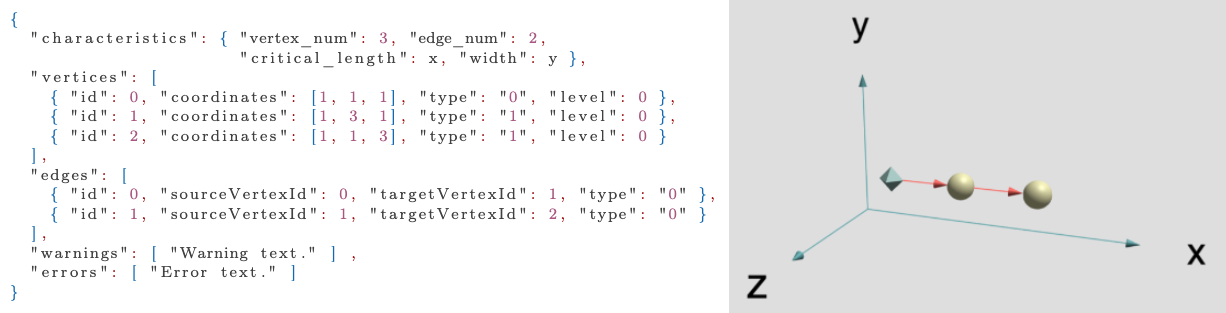
\includegraphics[height=3.1cm]{assets/json_example.png}
\caption{JSON structure, an example of the original data format and an example of visualization of this graph.}
\label{fig1}
\end{figure}

\subsection{Standard for visualizing algorithm graphs}

The Algorithm Graph Visualization Standard is a standard first described in the AlgoWiki project as a guide consisting of a set of rules according to which it is recommended to display an algorithm graph. The existence of the standard is determined by the need to construct images of algorithm graphs in a generally accepted form, which will be understandable regardless of the tools used to depict the graph. With the advent of the AlgoView system as a universal way to generate images of algorithm graphs, many provisions in the standard require revision. Innovations in the standard concern automation of the process and relaxation of the strict requirements for the image of graphs.
 % Обзор существующих решений
\section{Research methods and build a solution}

\subsection{Overview of existing solutions for processing XML files}

\textbf{SAX and DOM parsers.}

There are two main approaches to parsing XML files --- DOM and SAX APIs (Application Programming Interface).

DOM analyzers process an XML file by first loading the data of this file into the program in the form of a DOM (Document Object Model) tree \cite{m6}. It is a representation of an HTML document as a tree of tags.

SAX (Simple API for XML) analyzers, in turn, carry out stream-based event processing of XML documents without loading data into the internal structures of the program \cite{m7}.

Libraries that offer a DOM APIs were considered as a target option, since thread processing is not required for this work.

\textbf{Libraries that provide DOM APIs for processing XML files.} The most used libraries for the C++ language that provide the DOM API are RapidXML, PugiXML, TinyXML \cite{m9}.

RapidXML is primarily focused on reducing execution time and is a stable and fast parser that runs at speeds approaching the speed of the \texttt{strlen} function (a function that calculates the length in bytes) running on the same data \cite{m10}.

PugiXML is a library that provides a highly traversable/modifiable DOM programming interface, an extremely fast parser, and the ability to access data along a given path \cite{m11}.

TinyXML is a minimal version for parsing XML file data and is not as fast as the previous two. This library was created for reasons of ease of use and learning, and is well suited if high execution speed is not a priority factor when choosing tools for work \cite{m12}.

\textbf{Data binding compiler.} In addition to SAX and DOM analyzers, there is a way to process it using the XSD Schema data binding compiler. This method was proposed by Code Synthesis as an alternative solution for processing XML files with some advantages over traditional approaches \cite{m14}. Given an XML instance specification (XML Schema), it generates C++ classes representing the given vocabulary, as well as XML parsing and serialization code. Compared to APIs such as DOM and SAX, XML data binding allows the user to access data in XML documents using a generated domain vocabulary rather than generic elements, attributes, and text.

\textbf{Additional solutions for processing XML files.} In addition to the methods of working directly with XML files, it is possible to perform the same actions (access/analysis/processing) with data, only by first converting the XML format to JSON (JavaScript Object Notation) --- a standard text format for data exchange. In this case, libraries for working with the JSON format are already used to process the data, the most used of which is RapidJSON.

The method of presenting data when working with the DOM programming interface turned out to be important within the framework of this work. RapidJSON works with the Value entity, which can be of two types --- Object and Array. From the point of view of the source XML file, all its tags are objects and all tags of the same name are combined into arrays. Thus, the tree structure in which data is stored in the program in the RapidJSON library differs from the structures of libraries that work directly with the XML format \cite{m15}. And then bypassing this tree structure, and in particular the transition between tags of different names located at the same depth, is different and seems more convenient and safer from the point of view of memory access.

\subsection{Overview of libraries for calculating the values of mathematical expressions}

As part of the operation of the visualization system, there is a need to calculate and evaluate mathematical expressions that describe the information structure of the algorithm. For these purposes, in the C++ language, there is a set of third-party open source libraries implemented into projects. The most used and suitable for this work are ExprTk, muParser, METL (Math Expression Toolkit Library).

\textbf{ExprTk library.} ExprTk is the most complete and used library for parsing and evaluating the mathematical expressions above. The parsing engine supports many forms of functional and logical processing semantics and is easily extensible. The ExprTk library allows you to work with scalar, string and vector data types with numeric types Float, Double and MPFR (multiple-precision floating-point) and supports processing various mathematical operations and functions \cite{m17}. ExprTk works on the principle of parsing an expression in an AST tree, which allows you to evaluate its value. According to performance tests, the library is considered the fastest solution for computing standard operations with scalar values.

\textbf{MuParser library series.} MuParser is a series of extensible, high-perfor- mance libraries that provide the user with different capabilities depending on his needs \cite{m19}. To achieve greater speed of working with scalar values with restrictions on the number and type of parameters used and the accuracy of calculations, the muParserSSE library is used. To overcome these limitations with increasing operating time, muParser is used. To work with vector and string data types and complex numbers, the muParserX library version is applicable.

\textbf{METL library.} Math Expression Toolkit Library is a small library for the C++14 language standard for parsing mathematical expressions. It is designed to be flexible yet effective at the same time. Flexibility means that expressions can use all types of variables with reasonable behavior (useful for working with vectors and matrices, for example) and yet adding and editing operators and functions is very easy.

\textbf{Comparison of libraries.} The libraries were compared using performance tests designed to test the correctness of calculations and the speed of operation of libraries for parsing mathematical expressions written in C++ and working on the POEM (Parse Once Evaluate Many times) principle \cite{m22}. Based on the results of calculation time measurements, the leaders among libraries for parsing mathematical expressions are muParserSSE and ExprTkFloat, working with the Float data type, and taking into account the accuracy of calculations, ExprTk, working with the Double data type.

\subsection{Research on 3D visualization methods} 3D visualization is an important aspect of user experience in software development. Currently, there is a lot of research being done in the field of graph visualizations \cite{m23,m24,m25,m26,m27}. However, analyzing the performance of algorithms using information graphs is not a very popular area in science and does not contain established methods. Understanding how to implement a project requires further consideration of the popular 3D imaging technologies available today. During the study of available 3D visualization methods, about 10 different solutions were considered: OpenGL \cite{m28}, WebGL \cite{m29,m30,m31}, Three.js \cite{m32,m33}, Babylon.js \cite{m34}, VTK (Visualization Toolkit) \cite{m35}, OpenSceneGraph \cite{m36}, DirectX \cite{m37}, Unity \cite{m38}, Blender \cite{m39}, Maya \cite{m40}.

After a comparative analysis of visualization tools, it was concluded that the simplest and most convenient methods for visualizing graphs are implemented in the Three.js, Babylon.js frameworks, as well as on the Unity platform. The final choice was made in favor of the Three.js framework due to its lightweight and cross-browser compatibility. The OrbitControls module was used to control the scene. This module is the most common and supported solution for implementing control using a computer mouse and keyboard \cite{m43}. To create a user interface and control menu with capabilities for additional analysis of algorithm graphs, the lightweight dat.GUI module was used \cite{m44}. The size of the library with all additional user interface modules does not exceed 1 megabyte.

\subsection{Method of bending edges in three-dimensional space}

\textbf{Indicator of the need to bend edges.} The main signal for the need to bend the edge occurs when the vertex is crossed by a straight edge, since in this case it is often unclear where the edge comes from and where it goes. The intersection of different edges or the passage of an edge through the shell of a 3D vertex object on average does not create problems with the visual perception of the information graph.

\textbf{The mathematical meaning of edge bending.}  Let the three-dimensional Cartesian coordinate system $\Phi$ with basis vectors $\overrightarrow{i}, \overrightarrow{j}, \overrightarrow{k}$ have 2 vertices: $A(x_1; y_1; z_1)$ and $B(x_2; y_2; z_2)$. Let us denote the length of the vector $\overrightarrow{AB}$ as $len = \sqrt{
(x_2 - x_1)^2 +
(y_2 - y_1)^2 +
(z_2 - z_1)^2 }$. Let there be a segment between vertices $A$ and $B$ that needs to be geometrically bent. By bending the edge between the vertices we can imagine that the vector $\overrightarrow{AB}$ is one of the basis vectors of another three-dimensional Cartesian coordinate system $\Psi$, in which we need to describe the equation of the curve emanating from the point $A(0; 0; 0)$, that is, the origin of coordinates, and arriving at the point $B\left(len; 0; 0 \right)$, distant from the origin of coordinates at a distance of $len$. After describing the equation of the curve, we can go to the original basis, which positions the curve in space so that it corresponds to the vertices  $A$ and $B$ in the original coordinate system $\Phi$.

\textbf{Geometric method for finding the basis.} The vector $\overrightarrow{AB}$ in the three-dimensional coordinate system $\Phi$ corresponds to the segment $AB$ and is one of the basis vectors in the coordinate system $\Psi$. Let's calculate the first unit basis vector $\overrightarrow{n_1}$:

$$
\overrightarrow{n_1} = \frac
{\overrightarrow{AB}}
{\left|\overrightarrow{AB}\right|}
$$

To find the second unit basis vector $\overrightarrow{n_2}$ we will use geometric and trigonometric methods:

$$
b = \frac
{\left|y_{n_1}\right|}
{\tan\left(
\frac{\pi}{2}
-\sin(\left|x_{n_1}\right|)
\right)};
\quad
\gamma = \arctan\left(
\left|
\frac{z_{n_1}}{x_{n_1}}
\right|
\right);
$$

$$
\overrightarrow{n_2} = \left\{
-b\cos(\gamma)
\frac{x_{n_1}}
{\left|x_{n_1}\right|};
\quad
y_{n_1};
\quad
-b\sin(\gamma)
\frac{z_{n_1}}
{\left|z_{n_1}\right|}
\right\}
$$

To find the third unit basis vector $\overrightarrow{n_3}$ we use the vector product:

$$
\overrightarrow{n_3} = \overrightarrow{n_1} \times \overrightarrow{n_2}
$$

The unit vectors $\{\overrightarrow{n_1}, \overrightarrow{n_2}, \overrightarrow{n_3}\}$ form the basis of the three-dimensional Cartesian coordinate system $\Psi$.

\textbf{Method of bending edges through a parametrically defined circle.} The bending of the edge by finding the parametric equation of the curve occurs in the above-described three-dimensional Cartesian coordinate system $\Psi$. The optimal type of curved edge is the part of the circle bounded by the points $A(0; 0; 0)$, $B\left(len; 0; 0 \right)$. To obtain the desired edge, it is enough to use the standard method of finding the equation of a circle at a given center and radius.

$$
x = R\cos\theta + x_{center};
\quad
y = R\sin\theta + y_{center}
$$

The radius of the circumscribed circle $R$ has a linear dependence on the distance $len$. The center of the circle $C(x_{center}; y_{center}; 0)$ and the range of values of the parameter $\theta$ are calculated geometrically. % Исследование и построение решения задачи
\section{Construction of the architecture and algorithm of operation of the AlgoView system, software implementation}

\subsection{AlgoView system operation diagram}

The application consists of many steps that occur automatically. Let's consider the sequence of system actions, starting from loading into the system a file describing the information structure of the algorithm in the Algolang language, to obtaining an interactive 3D model of the information graph of this algorithm.

\textbf{Operation of the computational subroutine.} As input data, the system accepts a description of algorithms in the Algolang language in XML format. Next, the source file is converted into JSON format. The next step, using the RapidJSON library, is to create a DOM tree structure in memory, through which all the data in the original XML file can be accessed. This structure is traversed in order to collect all information about the graph into program classes with performing some intermediate calculations for ease of use, namely, calculating ranges of iteration space values. To calculate the values of these expressions, the ExprTk library is used. It is impossible to calculate all the expressions available in the description of the algorithm at this stage, since they depend on the current values of the iteration space and will be calculated in the future. When traversed, such expressions are stored as strings without modification as attributes of the class instance. After collecting all the data from the input file and carrying out preliminary processing, the main loop is launched, performing the meaningful work of the entire program. Inside it, a passage takes place throughout the entire iteration space, calculations are carried out that depend on its current values, the coordinates of the vertices are formed, their level of parallel form is determined \cite{m41}, and the vertices connected by an information edge are determined.

Based on the results of this stage, lists of instances of classes of vertices and edges with a description of their properties, general information about the graph and/or lists of warnings and errors (if any) are generated. Next, based on this information, a file with a JSON structure is generated as an intermediate data format, which is subsequently used to build an interactive 3D visualization.

\textbf{Operation of the visualization subroutine.} After creating the intermediate file, the user receives a web page with a visualization application that starts automatically after downloading. The first step is that the program converts the data from a JSON structure with intermediate data and composes the internal structure of the graph from them. Next, a 3D representation of the graph is created in the form of a set of 3D objects that correspond and visually describe all the structural elements of the graph. The last stage is the construction of an interactive visualization of the resulting set of 3D models, forming, together with the user interface, a multifunctional analysis system.

\subsection{Stages of the computational subroutine}

First, let's make a few disclaimers. In the process of describing the operation of the computational part of the visualization system, the used concept of a parallel form of an information graph will imply precisely the canonical NPL of this graph. The information graph of the algorithm, constructed as a result of the program, is not such in its classical sense, since it also contains vertices with input data, which contradicts the definition in which only the operations of the algorithm are vertices. That is, the concept of a graph used within the framework of the implemented program is, as it were, an epigraph formed by adding vertices with input data to the graph of the algorithm. There is also a restriction imposed on the input data, namely, for algorithm blocks (the \texttt{block} tag in the Algolang language) that describe the support polytopes of its graph, a restriction is imposed on no more than three-dimensional dimensions.

\textbf{Convert to JSON.} At the first stage of work, the XML file is instantly converted into JSON using the small xml2json library. Thus, an error handled by this step can only be an incorrect XML file structure.

\textbf{Collect input data.} The input collection phase uses the DOM API provided by the RapidJSON library to traverse the input file. The library was chosen due to its safer way of accessing the vertices of the DOM tree, built on the basis of XML, which eliminated the problems of jumping to a null pointer that arose with the Algolang language. As a result of traversing the DOM tree, program classes are created that contain all the necessary information about the information structure of the algorithm. The library also has built-in error handling tools, which were used to implement input data validation (for example, reusing an argument name within one block, setting incorrect argument boundaries, etc.).

\textbf{Evaluate mathematical and conditional expressions.} The ability to evaluate mathematical and conditional expressions is necessary to process the expressions described in the input data. The ExprTk library was chosen as a tool for these purposes, which is easily integrated into projects and offers a large base of processed functions and operations, and also quickly performs calculations. All calculations in the program are carried out by one separate function, which takes as input an expression in the form of a string and a map of the names and values of the parameters involved in the calculation.

\textbf{Main loop.} The so-called “Main loop” of the program carries out its content and forms program classes with final information about the algorithm graph model, which need only be rewritten in some standard form for further visualization. The operation of the “Main loop” implements the processing of one block of the algorithm; accordingly, this fragment of the program also works in a loop for all blocks. When a block is submitted for processing as a program class with all the information about it, a field of id numbers of the vertices of the future information graph is created based on the ranges of the iteration space and the shift of all coordinates along one axis is determined depending on the dimension of the previous block, so that the blocks do not overlap each other on a friend. At each iteration step, the current coordinate value is selected. Next, the cycle checks the conditions for the existence of vertices using the function of calculating mathematical expressions for these coordinates. If the condition is met, then a vertex is created for these values, which is assigned the next ordinal id and, based on the information obtained from the description in the Algolang language, its type, or, if the type was not specified, then it is assigned a default value. After this, all source vertices from which the edge leads to the current one are processed. It is checked whether this vertex exists by searching for it in the field of id-numbers of the vertices of the block to which it belongs, at the given coordinates. If such a vertex does not exist, then it is not an operation of the algorithm, but indicates a dependence on the input data. Such a vertex is created with a specially defined type of input data (type "0") and the level value of the parallel form of this vertex is assigned zero. If such a vertex existed, then from its coordinates the program obtains id, also referring to the field of vertices. After this, for each source vertex, based on its id and the id of the current vertex, an edge is created. After processing all source vertices, for the current vertex it is possible to determine the level of its parallel shape. Then the next iteration of the loop occurs.

\textbf{Generation of intermediate output data.} As a result of the operation of the “main loop”, the program generates a list of objects of program classes of vertices and edges with a description of their properties. Based on these lists, output data is generated in JSON format. Thus, the output of the implemented program is a list of vertices and edges with a listing of their properties, a listing of graph properties, and a listing of errors and/or warnings (if any). For Vertices - this is id, coordinates, type and level of the parallel form, for edges - id, id of the vertices that it connects, with the direction from the first named vertex to the second, and type, for a graph - the number of vertices and edges, the length of the critical paths and width of parallel form.

\textbf{Calculation of parallel form.} One of the most important capabilities of the system is to display the membership of groups of vertices to levels in a parallel form. This allows you to analyze which operations of the algorithm can be performed independently of each other (in parallel, in one time). The determination of the parallel form level for each vertex occurs, as mentioned earlier, within the framework of the “Main loop” according to the following principle:

\begin{enumerate}
    \item When creating a new vertex, the default value is level 0 of the tier-parallel form, which means that it does not belong to any tier, that is, it is not an operation (this type of vertex is the input data vertex)
    \item It is determined whether a given vertex is an operation or an input data, and in the second case it is assigned level 1 of the parallel form
    \item Data is collected on the level of the parallel form of all source vertices, if any, and the level of the current vertex is calculated using the formula
    $$ level = \max\left\{level(v): v \in source\_vertices\right\} + 1 $$
\end{enumerate}

\textbf{Analyze the graph to generate a list of errors and warnings.} The system is capable of analyzing and processing three types of errors. System critical errors notify the user that a system error has occurred and he cannot influence the result of the program. This type of error occurs rarely and is intended for the developer. Custom critical errors notify the user why the input data cannot be processed. The user can change the contents of the input files to eliminate errors. Non-critical errors resulting from the operation of the visualization system return a graph constructed in accordance with the XML description of the graph, but with the possible presence of errors in it, about which the user receives a warning.

\textbf{The principle of arrangement of vertices and edges in space.} To locate the vertices and edges of the information graph of the algorithm in three-dimensional space, the following principle was chosen. A three-dimensional Cartesian coordinate system and a fixed-size grid on it are introduced, depending on the range of values of the iteration space. Further, any vertex of the algorithm graph is located in a unique grid node and is specified by the coordinates of this node. Any edge is defined by a pair of grid nodes - its beginning and end. In this way, any information graph of the algorithm can be displayed in three-dimensional space without overlapping vertices. To determine whether a vertex belongs to the level of a parallel form, means of interactive visualization of the final model are used.

\subsection{A software architecture for the visualization task}

One of the main tasks when implementing a system in software is the selection and development of a suitable application architecture. The chosen architecture determines the way data is processed and communicates with the user. Choosing an inappropriate structure and methods for communicating application modules with each other can significantly increase the load on the browser kernel and the operating system's computing resources. Let's consider the main modules of the visualization system to solve this problem:

\begin{enumerate}
    \item Working with data, reading and creating the internal structure of the graph.
    \item Working with the graph structure based on the view parameters specified by the user. Creation of 3D models for each object in the graph structure.
    \item Creation of a 3D scene containing a graph model.
    \item Working with the user: ensuring communication of the control panel with the graph model, scene and parameters and view.
    \item When changing view parameters, the data in the model must change locally and consistently update the structure of the graph and the 3D model representing this graph on the stage.
\end{enumerate}

The described requirements and main functional parts are sufficient criteria for choosing a Model-View-Controller (MVC) architecture \cite{m45}.

\textbf{Description of the MVC architecture used.} MVC architecture is a pattern for software implementation that divides the application's data handling, user interface, and control logic into three interconnected independent components. The Model represents the data and business logic of the application, the View represents the presentation layer of the application, and the Controller acts as an intermediary between the Model and the View, processing user input and updating the Model and View as needed. When the user interacts with the application, the controller receives the input and decides how to update the model and view accordingly. The Model is responsible for processing the data and updating itself, and the View displays the data to the user in a presentable format. This architecture helps break complex applications into smaller, more manageable components, making the application easier to develop, test, and maintain \cite{m46}.

\textbf{Separation of responsibilities between modules of the AlgoView visualization system.} In the AlgoView visualization system under consideration, the MVC architecture used consists of a model (Model) with a graph structure, a display part (View) with a set of methods for converting data into 3D models, and a controller (Controller) containing methods for changing the model and updating visualization through the user interface. Having chosen an architecture, you need to correctly distribute tasks and responsibilities between application modules, following the rules of a specific architecture. Let's consider how responsibility is distributed in this case:

\textit{Contents of the Model module}: processing of input data; storing the internal structure of the graph; updating data in the graph structure based on user commands.

\textit{Contents of the View module}: providing a set of methods for converting data into 3D models; filling the scene with 3D models obtained from graph objects stored in Model.

\textit{Contents of the Controller module}: creation of a graphical user interface; ensuring communication between the user, his commands through the control menu and the Model-View link; managing Model and View through their built-in control methods. % Описание Экспериментальной части
\section{Example of AlgoView system operation}

Let's look at an example of how the system works using a simple algorithm: ``Finding the sum of array elements by doubling'' (fig.~\ref{fig2}). The doubling method is used as a fast option for computing long sequences of associative operations. Elements at each stage of the algorithm are divided into pairs. Each pair contains the sum of its constituent elements. At the next stage, these sums are divided into pairs, etc. Characteristics of the algorithm (for summing an array of order n): total number of vertices: $n-1$; critical path length: $\left\lceil{\log_2n}\right\rceil$; canonical width of the parallel form: $n$.

\textbf{Sequential complexity of the algorithm.} To calculate the sum of an array consisting of $n$ elements, for any decomposition of $n$ into pairs, the essence of the algorithm comes down to a simple rearrangement of parentheses in the summation formula. The number of operations is constant and equal to $n-1$. A sequential algorithm should be classified as a \textit{linear complexity} algorithm based on the number of sequential operations.

\textbf{Algorithm parallelism resource.} To sum an array of order $n$ using the doubling method in the parallel version, it is necessary to sequentially execute $\left\lceil{\log_2n}\right\rceil$ tiers with decreasing ones (from $n/2$ to 1) number of summation operations. When classifying by the height of the parallel form, the doubling method therefore refers to algorithms with \textit{logarithmic complexity}. When classified by the width of the parallel form, its complexity will be \textit{linear}.


\begin{figure}
% \vspace{-0.5cm}
\centering
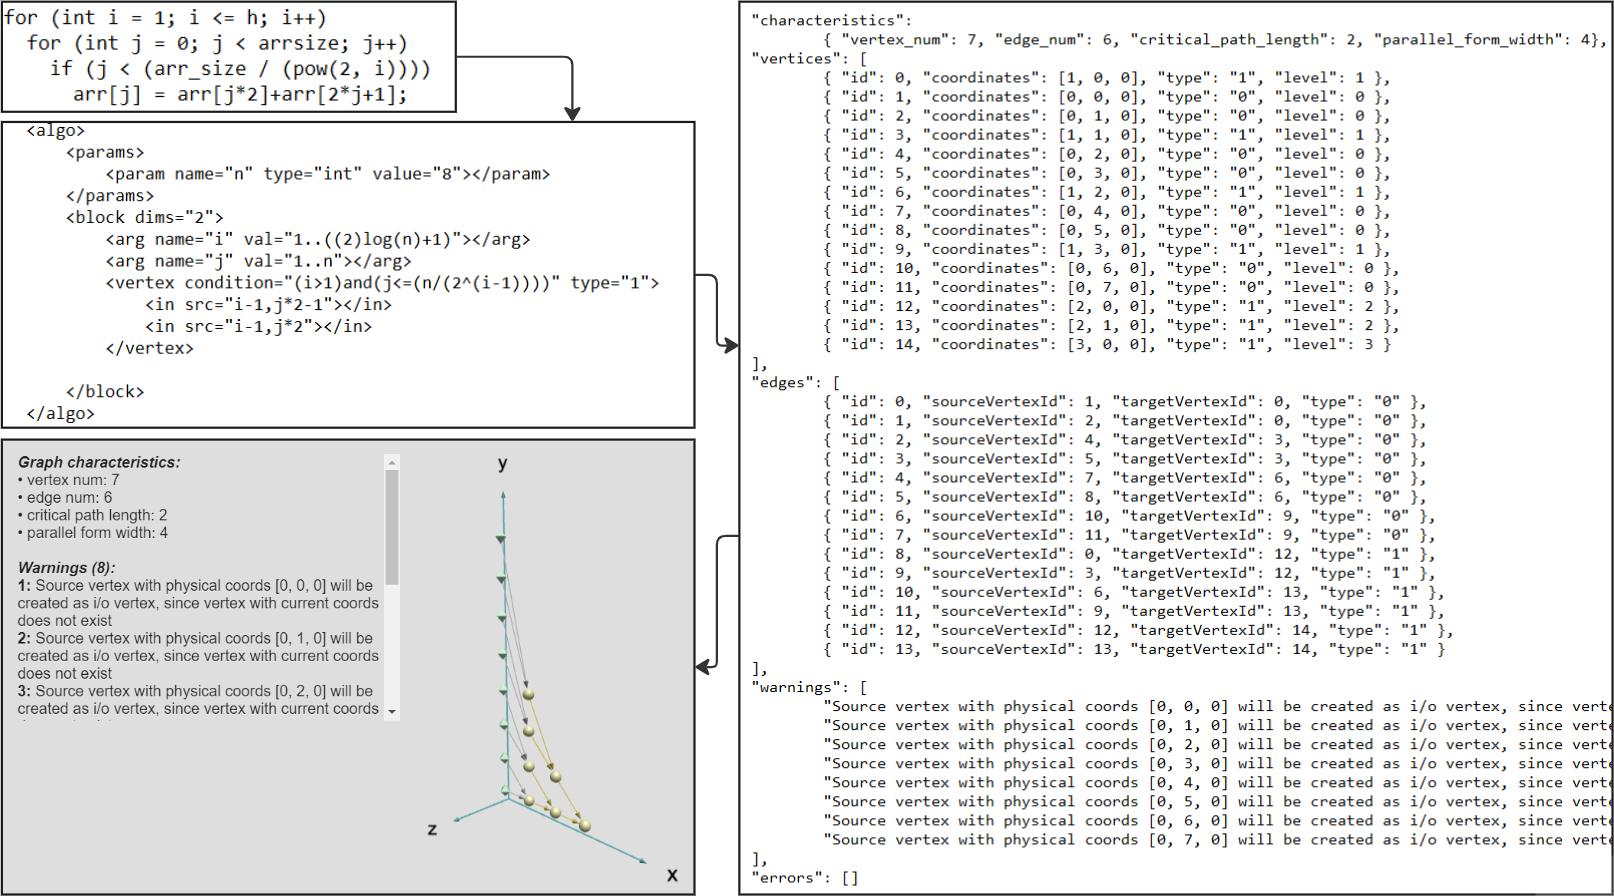
\includegraphics[height=6.78cm]{assets/algo_example.png}
\caption{Operation of the AlgoView system using the example of the algorithm ``Finding the sum of array elements by doubling'' for $n = 8$ from the implementation of the algorithm in the C language to the final visualization.}
\label{fig2}
\end{figure} % Заключение

\nocite{*}
\bibliographystyle{gost71u} % Для соответствия требованиям об оформлении списка литературы
\bibliography{references}

% \section*{Приложение}
\addcontentsline{toc}{section}{Приложение}
\label{sec:Apendix} \index{Apendix}

 

\end{document}
